\subsection{\label{sec:analysis} Analysis}
In this section, we perform an analysis of exactly how DDS is learning, and what kind of data it is learning to select.
We focuse particularly on multilingual NMT, because in this case the choice of data directly corresponds to picking a language, which has an intuitive interpretation.
\begin{center}
  \includegraphics[width=0.245\columnwidth]{figs/aze_devppl_plot.eps}
  \includegraphics[width=0.23\columnwidth]{figs/bel_devppl_plot.eps}
  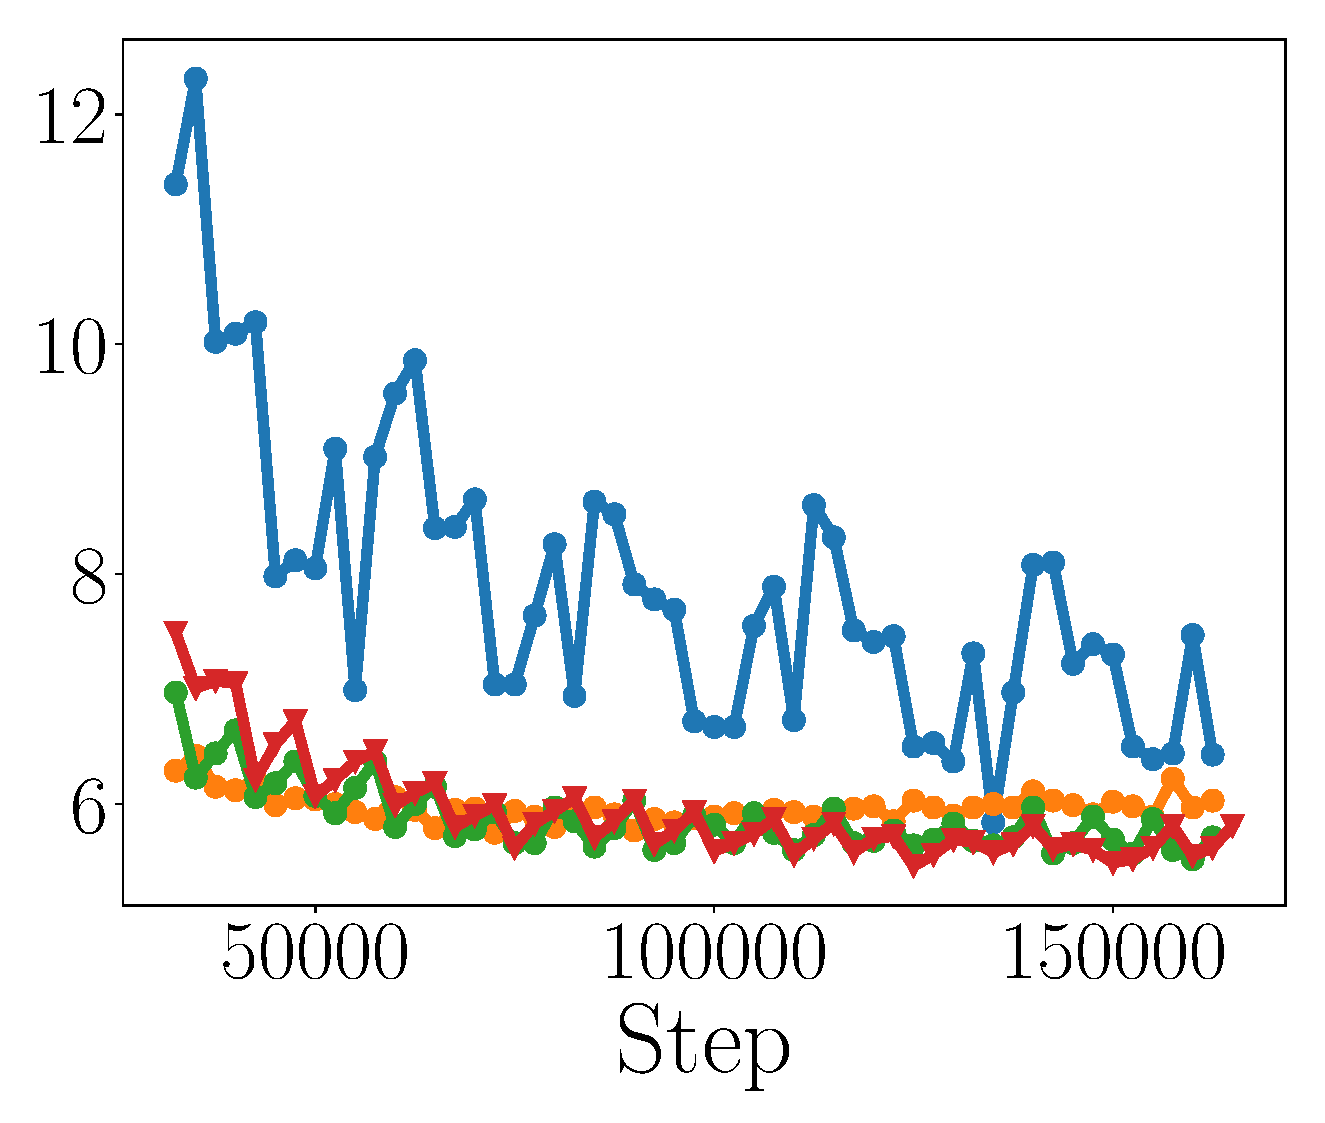
\includegraphics[width=0.23\columnwidth]{figs/glg_devppl_plot.eps}
  \includegraphics[width=0.23\columnwidth]{figs/slk_devppl_plot.eps}
  \captionof{figure}{\label{fig:nmt_converge}Development set perplexity vs. training steps. \textit{From left to right}: \texttt{aze}, \texttt{bel}, \texttt{glg}, \texttt{slk}.}
\end{center}
\paragraph{Training Curves.} First, we plot the dev set perplexity over the course of training in Figure \ref{fig:nmt_converge}.
DDS, with or without initialization with the heuristic distribution from TCS, allows the model to reach lower dev perplexity than TCS for all 4 languages.
\gn{Would like to add more here. How does ``Uniform'' compare? Explain that convergence is faster with initialization with TCS.}

\begin{center}
  \includegraphics[width=0.22\columnwidth]{figs/aze_hs_probs_plot.eps}
  \includegraphics[width=0.22\columnwidth]{figs/bel_hs_probs_plot.eps}
  \includegraphics[width=0.22\columnwidth]{figs/glg_hs_probs_plot.eps}
  \includegraphics[width=0.29\columnwidth]{figs/slk_hs_probs_plot.eps}
  \captionof{figure}{\label{fig:nmt_distrib_hs}Language usage for TCS$+$DDS by training step. \textit{From left to right}: \texttt{aze}, \texttt{bel}, \texttt{glg}, \texttt{slk}.}
\end{center}

\begin{center}
  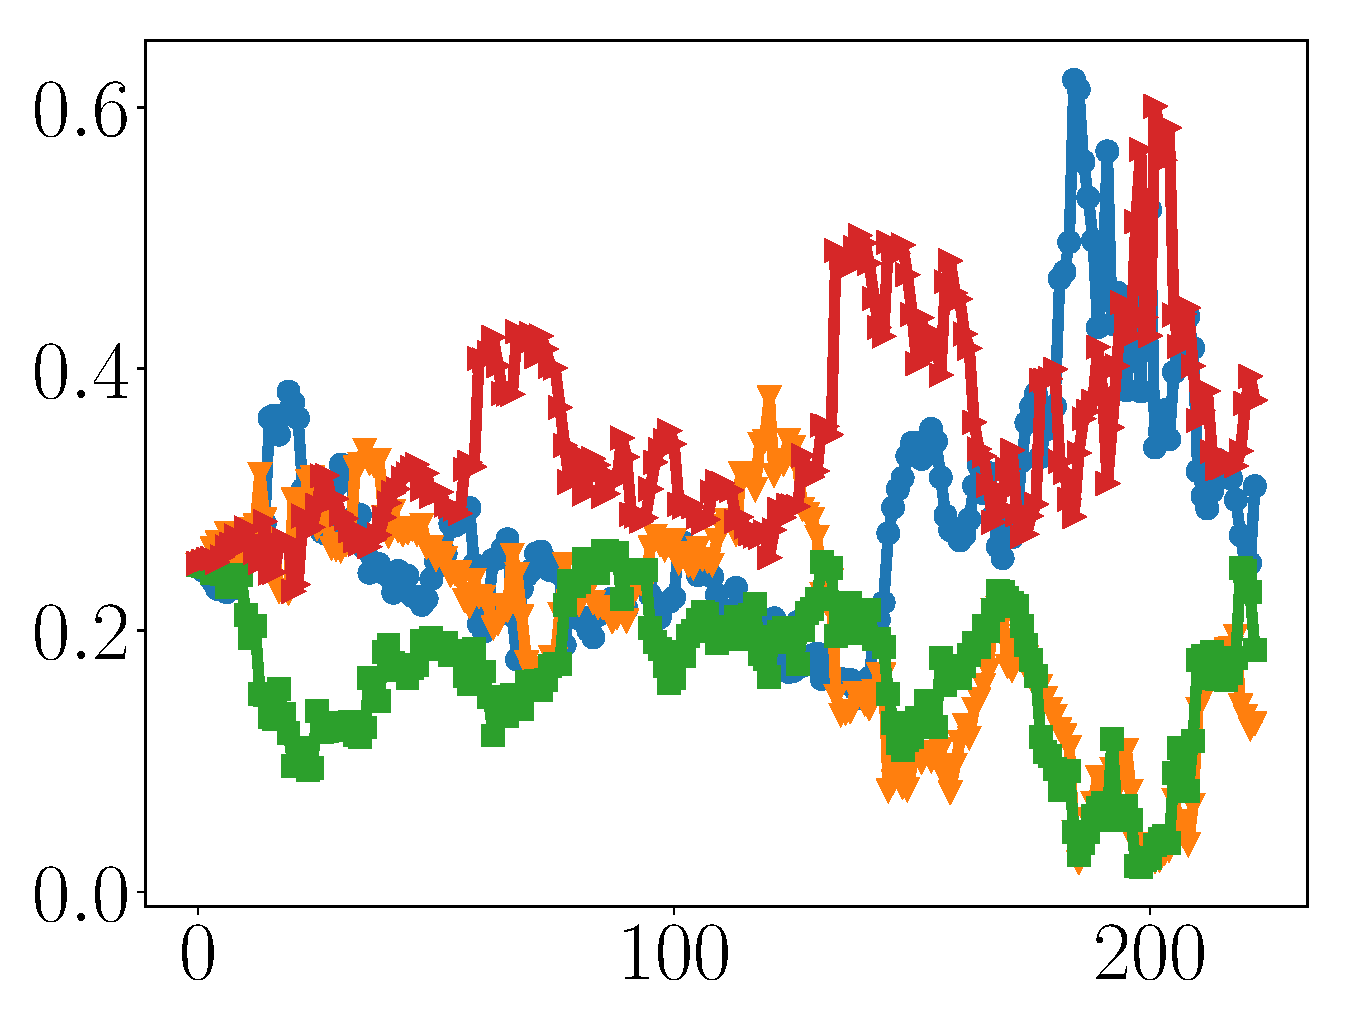
\includegraphics[width=0.22\columnwidth]{figs/aze_uni_probs_plot.eps}
  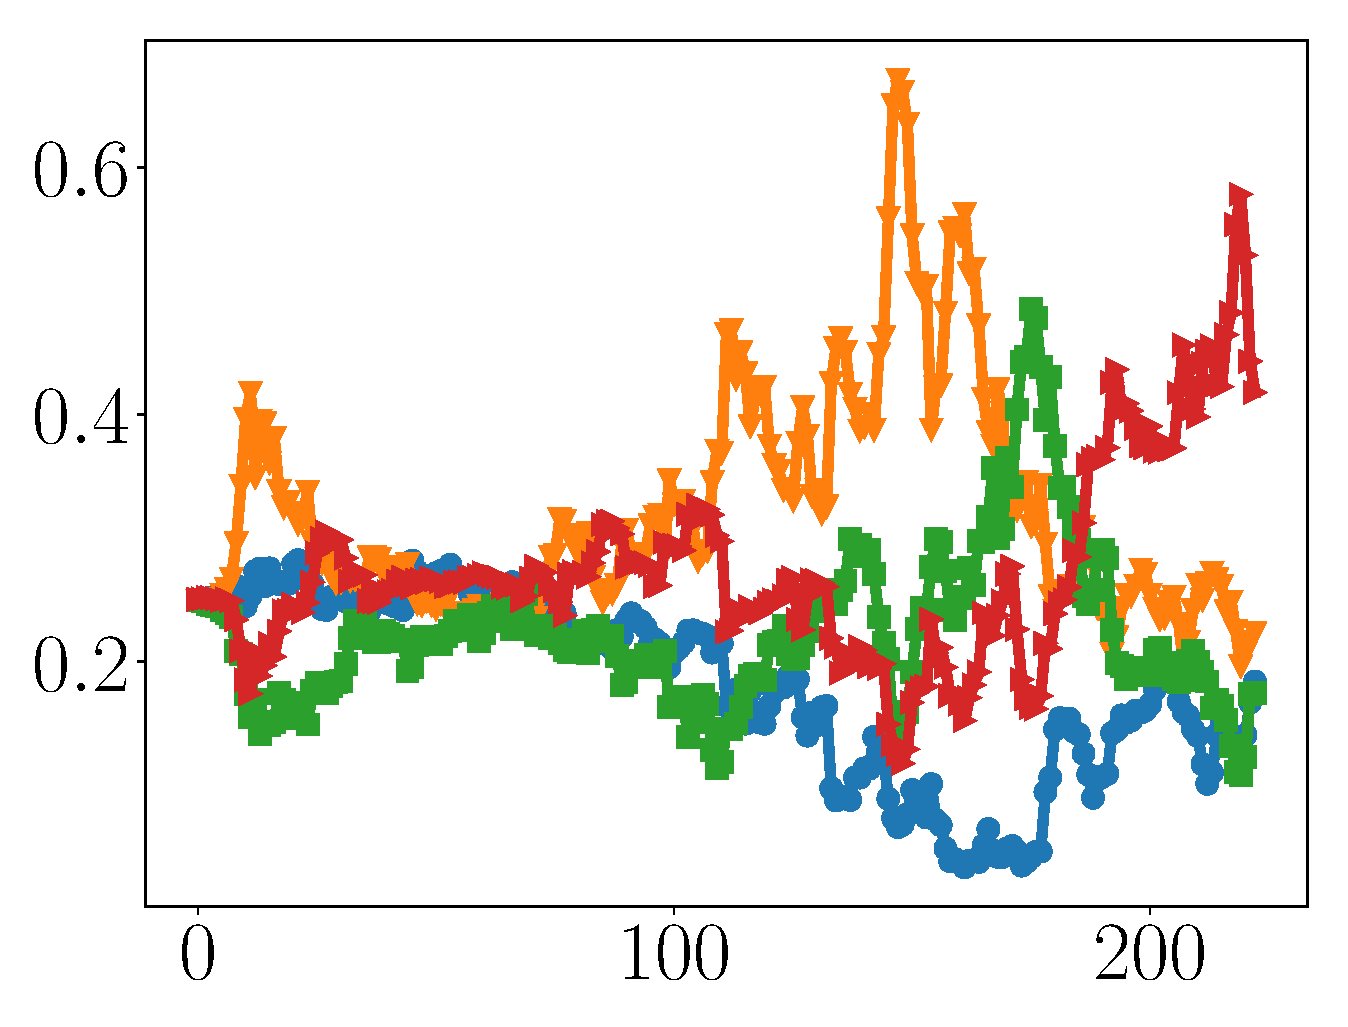
\includegraphics[width=0.22\columnwidth]{figs/bel_uni_probs_plot.eps}
  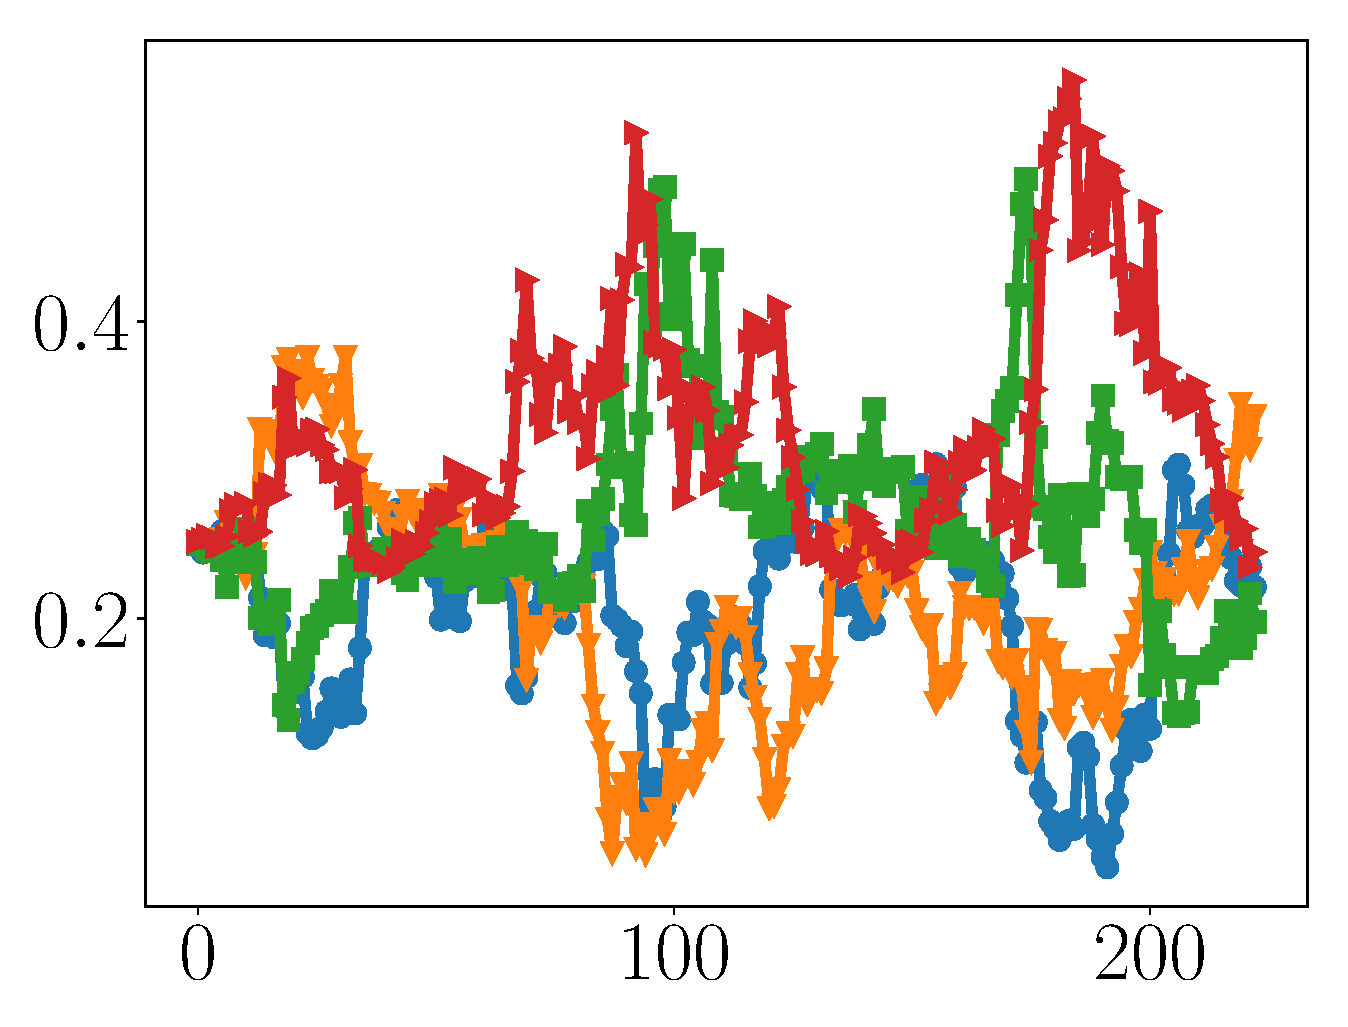
\includegraphics[width=0.22\columnwidth]{figs/glg_uni_probs_plot.eps}
  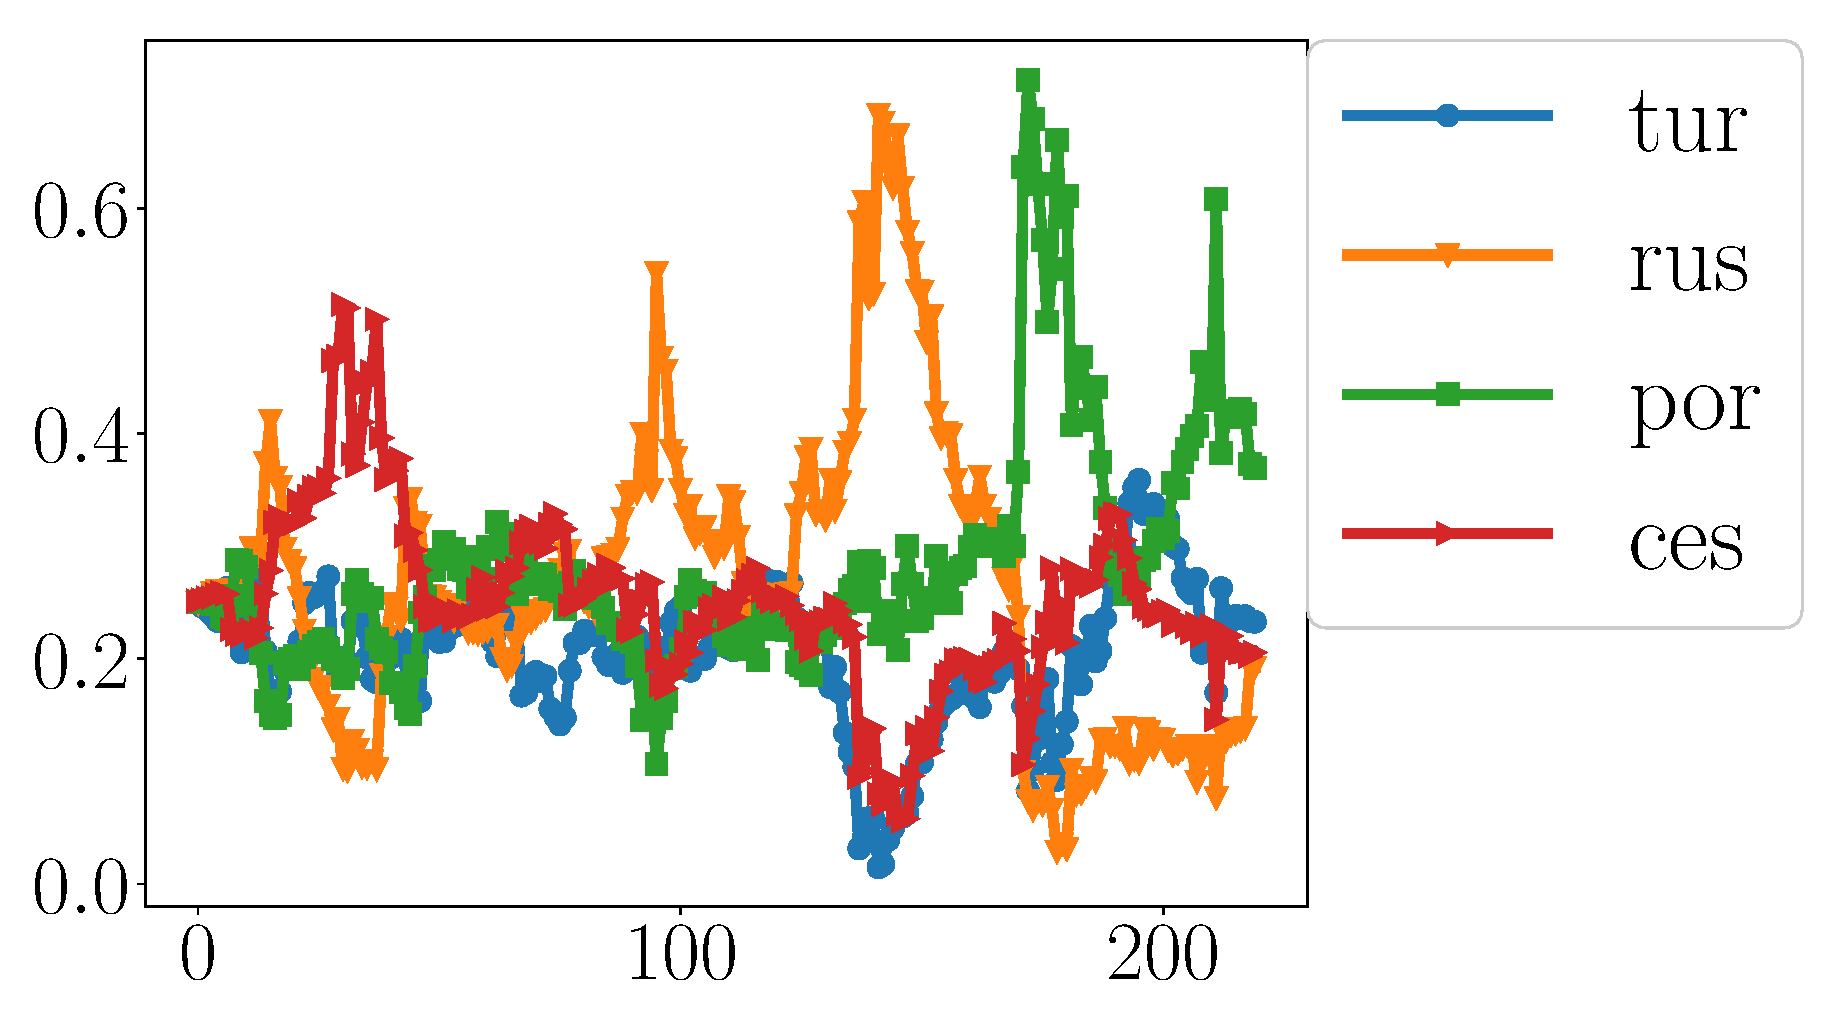
\includegraphics[width=0.29\columnwidth]{figs/slk_uni_probs_plot.eps}
  \captionof{figure}{\label{fig:nmt_distrib_uni}Language usage for DDS by training step. \textit{From left to right}: \texttt{aze}, \texttt{bel}, \texttt{glg}, \texttt{slk}.}
\end{center}
\paragraph{Learned Language Distributions.}
To analyze the learned language distribution, we plot the probability distribution of the four HRLs (because they have more data and thus larger impact on training) over the course of training.  Figure \ref{fig:nmt_distrib_hs} shows the change of language distribution for TCS+DDS. Since TCS selects the language with the largest vocabulary overlap with the LRL, the distribution is initialized to focus on the most related HRL. For all four LRLs, the percentage of their most related HRL start to decrease as training continues. For \texttt{aze}, DDS quickly comes back to using the its most related HRL. However, for \texttt{bel}, DDS continues the trend of using all four languages. This shows that DDS is able to maximize the benefits of the multilingual data by having a more balanced usage of all languages. 
%For gig and slk, DDS learns to mainly use both por and ces, their corresponding HRL.

In Figure \ref{fig:nmt_distrib_uni}, we show a more interesting trend of DDS without heuristic initialization.
For both \texttt{aze} and \texttt{bel}, our method learns to focus on their most related HRL after a certain number training updates.
Interestingly, for \texttt{bel}, DDS learns to focus on both \texttt{rus}, its most related HRL, and another language \texttt{ces}. Similarly for \texttt{slk}, DDS also learns to focus on \texttt{ces}, its most related HRL, and \texttt{rus}, although there is little vocabulary overlap between \texttt{slk} and \texttt{rus}.
Also notably, the ratios significantly change over the course of training, indicating that different types of data may be more useful during different stages of learning the model.
Notably, DDS shows significant improvements over uniform sampling and other heuristics, demonstrating that it is able to discover when it should use other data, even if the patterns are not immediately intuitive.
%Similar to the trend in Figure \ref{fig:nmt_distrib_hs}, glg tends to use both por, its most related HRL, and ces. 
